\documentclass[french]{article}
\usepackage[T1]{fontenc}
\usepackage[utf8]{inputenc}
\usepackage{lmodern}
\usepackage[a4paper]{geometry}
\usepackage{babel}
\usepackage{graphicx}
\begin{document}
\title{Rapport de Projet Uno}
\author{Anthony Boens, Bilel Aloui, Alexis Verhaeghe}
\date{\today}
\maketitle
\vfill 

\paragraph{Étudiants : Anthony Boens, Bilel Aloui, Alexis Verhaeghe}

\paragraph{Encadrant : Julien Dehos}

\paragraph{Date de début : \date{06 juin 2016}}

\paragraph{Date de fin : \date{22 juin 2016}}

\paragraph{Objet du projet : Jeu de carte Uno à 4 joueurs}

\tableofcontents


\section{Présentation du projet}
Notre projet consiste à créer un jeu de carte UNO à 4 joueurs en réseau avec une interface graphique.
Au lancement du jeu, un écran de login demande le pseudo et l'adresse IP du serveur.
Une fois que les 4 joueurs sont connectés, notre serveur distribue les cartes et la cartes du milieu. Un petit jeton indique la personne qui doit jouer et un petit compteur affiche le nombre de cartes des adversaires.
Une fois que qu'un joueur a posé sa dernière carte, le jeu s'arrête et affiche une image \og perdant\fg{} ou \og gagant\fg{}.
\subsection{Analyse de la demande}
La demande du client nous a imposé de faire le projet en C++ et la partie réseau et graphique en SFML. Le delais de réalisation du projet était de 3 semaines.
Les principaux besoins étaient de permettre à un joueur de se connecter sur un serveur et faire une partie en multijoueur de UNO avec toutes les règles du jeu respectées.
La première proirité était d'avoir un jeu fonctionnel comprenant toutes les règles (y compris les cartes changement de couleur), la seconde était de pouvoir jouer en réseau.

\subsection{Spécifications}
\textbf{Spécification serveur:}
\begin{enumerate}
	\item Lancement du serveur
	\item Stockage des clients
	\item Distribution des cartes
	\item Quand les 4 joueurs sont connectés, envoie de la carte courante (carte au milieu)
	\item Lancement du jeu (envoie de la demande de joueur au joueur)
	\item Mise à jour de la position du jeton qui indique quel joueur doit jouer
	\item Gestion des cartes spéciales
	\item Envoie de carte supplémentaire quand le joueur ne peut pas jouer
	\item Si le joueur ne peut toujours pas jouer, il passe son tour
\end{enumerate}

\textbf{Spécification client:}
\begin{enumerate}
	\item Lancement de la fenêtre de login
	\item Connexion au serveur si le formulaire est bien remplit (en appuyant sur la touche Entrée)
	\item Lancement de l'interface graphique du jeu
	\item Possibilité de cliquer uniquement sur les cartes \og jouables\fg{}
	\item Envoie de la carte choisit
	\item Affichage de l'image et fin du jeu quand un joueur n'a plus de cartes
\end{enumerate}

\section{Réalisation}
Le projet a entièrement été réalisé en C++ et plus précisement avec la bibliothèque SFML.

\subsection{Présentation} 
Le logiciel implémenté permet de charger un terminal qui lance un serveur (specification 1 du serveur) et affiche si les clients sont bien connectés (specification 2 du serveur). Dans la seconde fenêtre, on voit l'interface graphique du client avec les cartes distribuées mais pas la carte courante (specification 3 du client.
\begin{center}
\centering
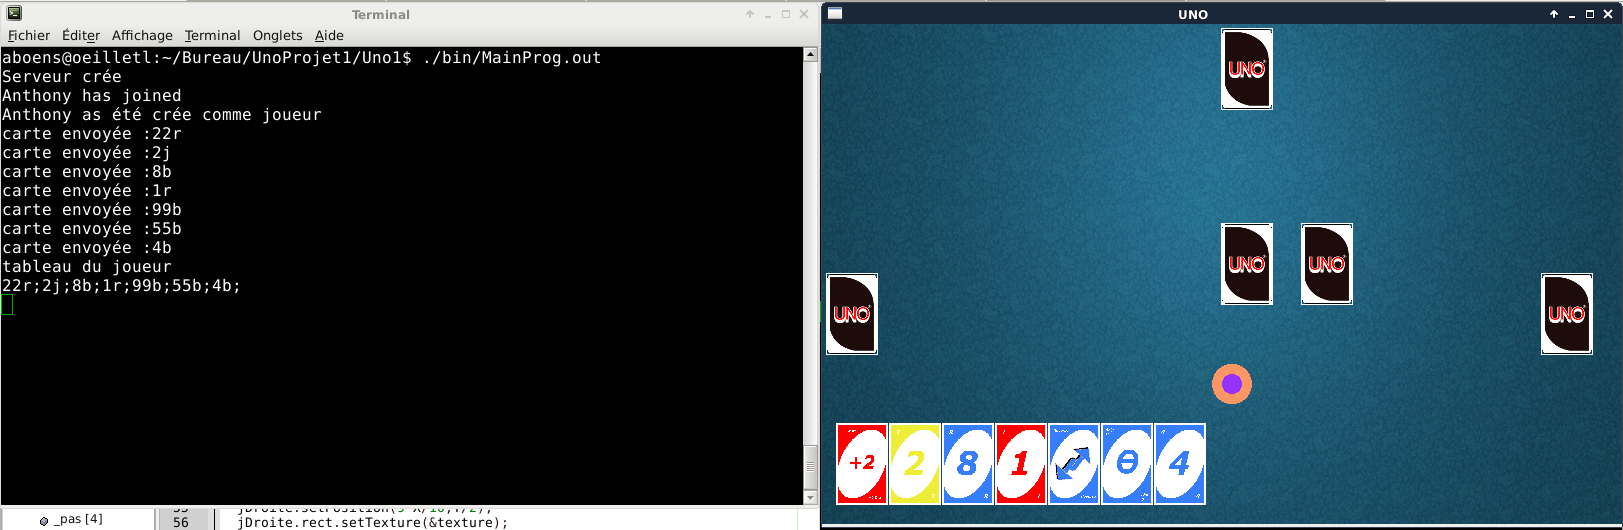
\includegraphics[width=0.7\linewidth]{cp}
\end{center}

Avant de lancer l'interface graphique du jeu, un écran de login apparaît et demande le pseudo et l'adresse IP du joueur (specification 1 du client). Le carré de connexion devient vert quand le formulaire est remplit et quand le client appuie sur la touche Entrée, le client envoie sont pseudo et se connecte au serveur (specification 2 du serveur).
\begin{center}
	\centering
	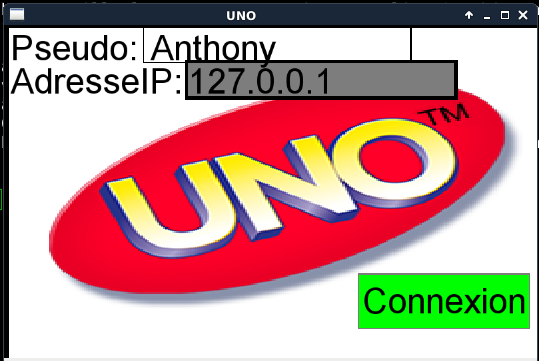
\includegraphics[width=0.7\linewidth]{login}
\end{center}

\subsection{Architecture générale}
\subsection{UML}
\begin{center}
	\centering
	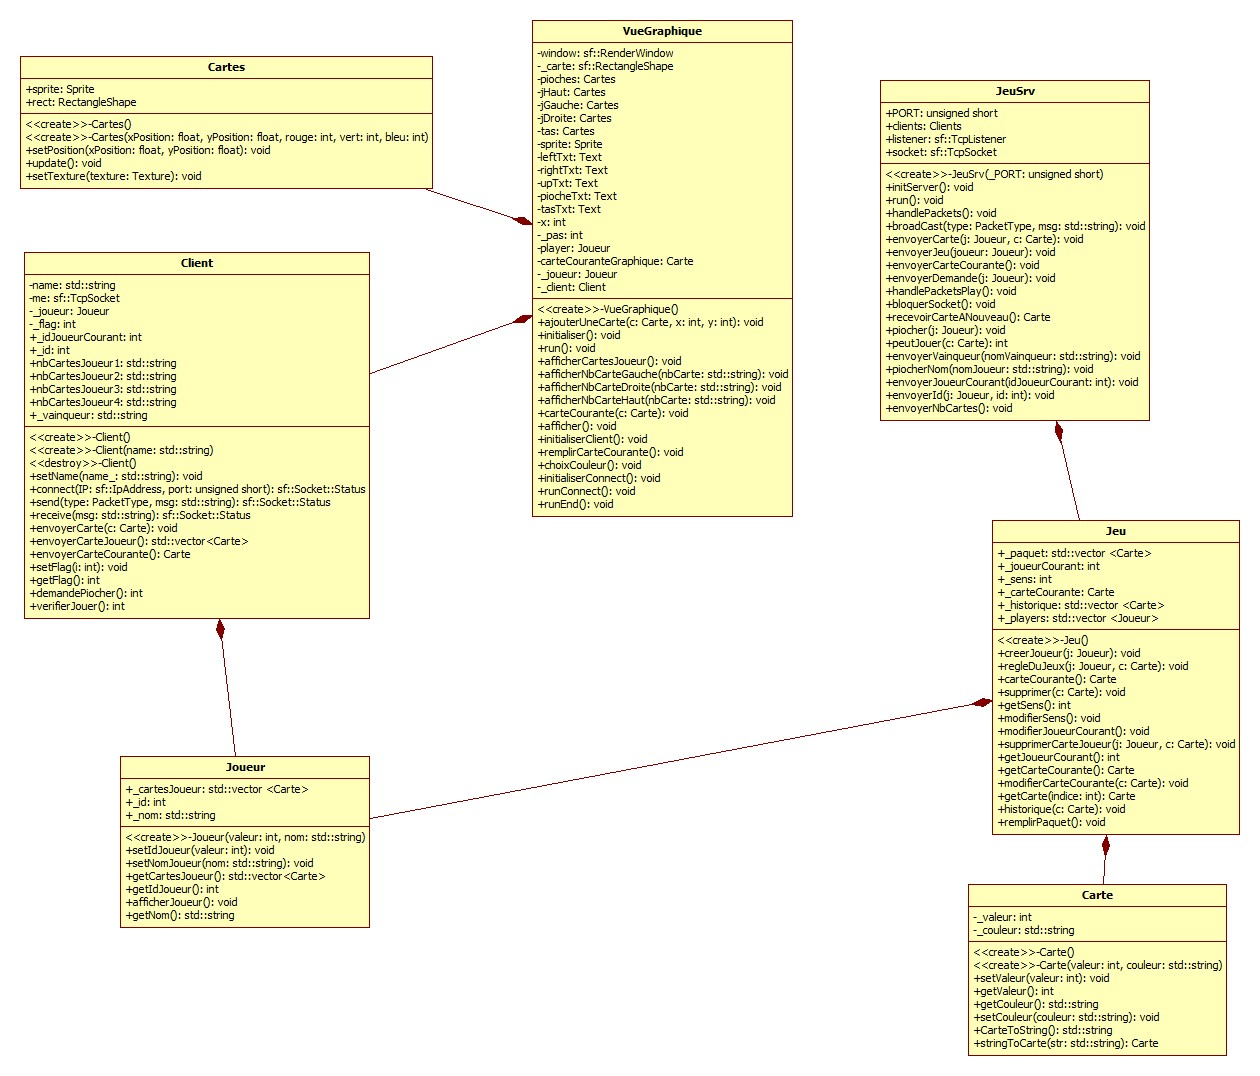
\includegraphics[width=0.7\linewidth]{uml}
\end{center}


\subsection{Cartes spécifiques}
\subsubsection{Les cartes changement de sens}
\begin{center}
\centering
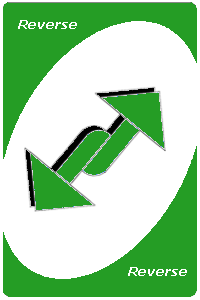
\includegraphics[width=1cm, height=2cm]{99v}

\includegraphics[width=1cm, height=2cm]{99b}
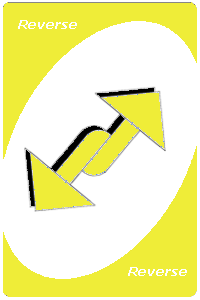
\includegraphics[width=1cm, height=2cm]{99j}

\includegraphics[width=1cm, height=2cm]{99r}
\end{center}
Ces cartes permettent de changement le sens du jeu. Si le jeu tourne dans le sens des aiguilles d'une montre, en jouant cette carte alors le jeu tournera dans le sens inverse.

\subsubsection{Les cartes passe-tour}
\begin{center}
	\centering
	
\includegraphics[width=1cm, height=2cm]{55v}
	
\includegraphics[width=1cm, height=2cm]{55b}
	
\includegraphics[width=1cm, height=2cm]{55j}
	
\includegraphics[width=1cm, height=2cm]{55r}
\end{center}
Si ces cartes sont jouées, le joueur suivant ne peut pas jouer, il passe son tour.

\subsubsection{Les cartes +2}
\begin{center}
	\centering
	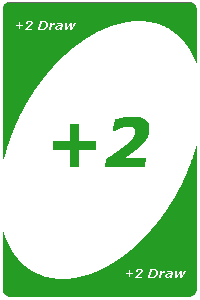
\includegraphics[width=1cm, height=2cm]{22v}
	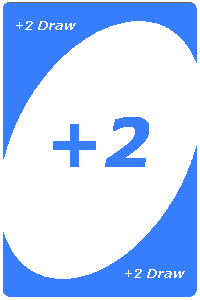
\includegraphics[width=1cm, height=2cm]{22b}
	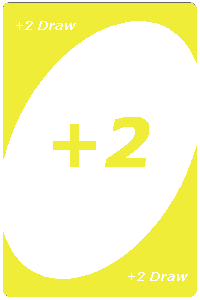
\includegraphics[width=1cm, height=2cm]{22j}
	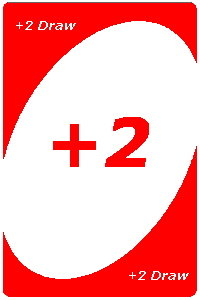
\includegraphics[width=1cm, height=2cm]{22r}
\end{center}
Si ces cartes sont jouées, le joueur suivant prend 2 cartes de plus dans son jeu. Il peut quand même jouer.

\subsubsection{Les cartes +4}
\begin{center}
	\centering
	
\includegraphics[width=1cm, height=2cm]{44n}
	
\includegraphics[width=1cm, height=2cm]{44v}
	
\includegraphics[width=1cm, height=2cm]{44b}
	
\includegraphics[width=1cm, height=2cm]{44j}
	
\includegraphics[width=1cm, height=2cm]{44r}
\end{center}
Cette carte peut être jouée peut importe le chiffre et la couleur de la carte courante.
Dans le jeu du joueur, la carte est noire à la base. Quand la carte est jouée alors un curseur apparaît et demande au joueur de choisir la couleur. En fonction de son choix, la carte courant change de couleur, le joueur suivant prend 4 cartes et il peut jouer si il a la même couleur.
\begin{center}
	\centering
	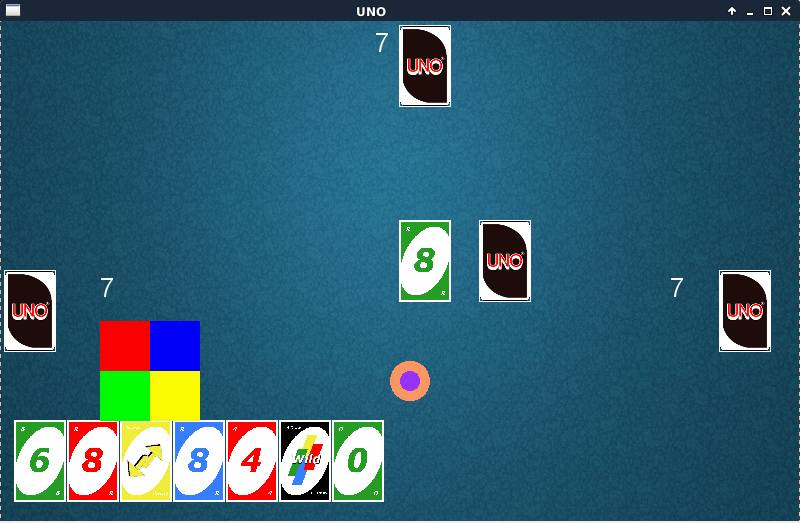
\includegraphics[width=6cm, height=4cm]{+4-curseur}
	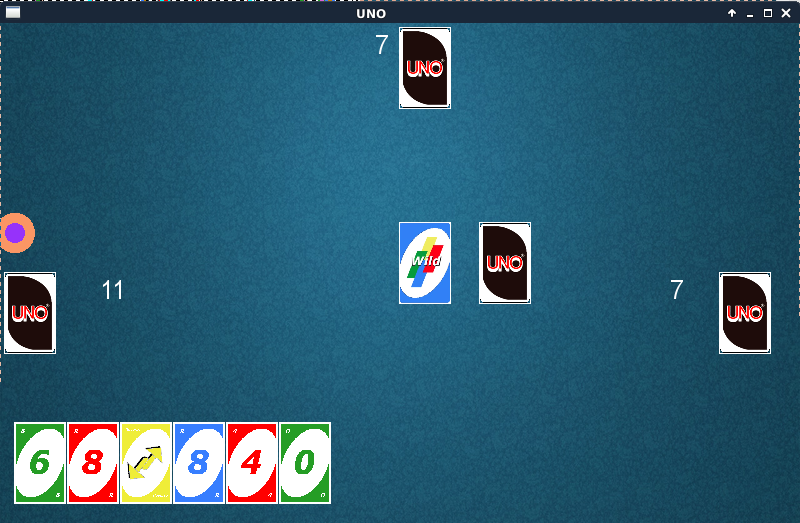
\includegraphics[width=6cm, height=4cm]{+4-bleu}
\end{center}
\subsubsection{Les cartes changement de couleur}
\begin{center}
	\centering
	
\includegraphics[width=1cm, height=2cm]{11n}
	
\includegraphics[width=1cm, height=2cm]{11v}
	
\includegraphics[width=1cm, height=2cm]{11b}
	
\includegraphics[width=1cm, height=2cm]{11j}
	
\includegraphics[width=1cm, height=2cm]{11r}
\end{center}
Cette carte peut être jouée peut importe le chiffre et la couleur de la carte courante.
Dans le jeu du joueur, la carte est noire à la base. Quand la carte est jouée alors un curseur apparaît et demande au joueur de choisir la couleur (même fonctionne que pour le carte +4).. En fonction de son choix, la carte courant change de couleur, le joueur suivant peut jouer si il a la même couleur.

\section{Bilan}
\subsection{Déroulement du projet}

Nous avons eu plusieurs différences par rapport à ce que nous avions prévu au départ, notamment sur le nombre de joueurs possibles. Au début nous envisagions de faire une partie entre 2 et 4 joueurs mais nous avons préféré de faire une partie uniquement à 4 joueurs pour des raisons techniques et par manque de temps. Nous avons aussi rencontré des problèmes pour assembler les codes de l'interface graphique, du réseau et des règles du jeu. En effet, chacun de nous travaillait sur une partie, indépendemment des autres pendant une semaine. Nous nous sommes rendu compte que ce n'était pas le bon choix donc la deuxième semaines nous avons travaillé ensemble pour comprendre le code de chacun et les associer. A ce moment, on a pu créer un jeu fonctionnel et se concentrer sur les problèmes techniques du jeu.
Au début du projet, nous avons voulu passé le pseudo de chaque client et l'adresse du serveur en argument lors de l'execution. Nous avons préféré créer un menu de login pour que notre code puisse être utilisé par un utilisateur lambda.

\subsection{Réalisation des objectifs}
\begin{tabular}{| l | c |}
	\hline
	fonctionnalité & réalisation \\
	\hline
	\hline
	Lancement du serveur et stockage des clients & complète \\
	\hline
	Distribution des cartes aux clients & complète \\
	\hline
	Envoie de la carte courante & complète \\
	\hline
	Lancement du jeu & complète \\
	\hline
	Interface graphique & complète \\
	\hline
	Jeton indiquant le joueur qui doit jouer & complète \\
	\hline
	Gestion des cartes spéciales & complète \\
	\hline
	Fenêtre de login & complète \\
	\hline
	Connexion au serveur avec une IP et enregistrement du pseudo & complète \\
	\hline
	Envoie des cartes vers le serveur & complète \\
	\hline
	Affichage de la fin du jeu & complète \\
	\hline
	Blocage de 4 connexions au serveur & Partielle \\
	\hline
	Possibilité de relancer une nouvelle partie & non \\
	\hline
	Possibilité de choisir le nombre de joueurs & non \\
	\hline
	
\end{tabular}

\subsection{Conclusion pour les projets futurs}
Pour les projets futurs, nous analyserons mieux la demande et feront un MVC mélangeant l'interface graphique, le réseau et le jeu avant de se lancer sur le code. Sinon c'est un projet qui nous a permit d'apprendre de nouvelles choses et surtout apprendre à travailler en groupe sur un projet commun.
\end{document}
